\section{Theoretical Analysis}
\label{sec:analysis}

In this section we will analyse theoretical our audio amplifier circuit. \\
To do so, and because there were several things to be analysed, we divided the theoretical analysis in the following subsections that explain the different sectors that our circuit has and also each one will be detailed separately.\\

The constants values used are expressed in the following table.

\begin{table}[H] \centering
\begin{tabular}{|
>{\columncolor[HTML]{FFCC67}}l |c|}
\hline
\multicolumn{2}{|l|}{\cellcolor[HTML]{EABD8B}Name - Value} \\ \hline
C1 & 7.500700e-04 F\\ \hline
C2 & 7.500700e-04 F\\ \hline
C3 & 6.499700e-04 F\\ \hline
RB1 & 3.999900e+04 Ohm \\ \hline
RB2 & 2.935300e+03 Ohm \\ \hline
RC & 4.999600e+03 Ohm\\ \hline
RE1 & 1.000070e+02 Ohm\\ \hline
RE2 & 5.995248e+02 Ohm\\ \hline

\end{tabular}
\caption{optab}
\end{table}

\subsection{Gain Stage}

In the first place, we must discuss the first half of the circuit that was used. The goal of the gain stage is to ensure a high input voltage so the input signal is not degradated or distorted throughout the circuit. It also has an elevated gain associated, so this is the part that is responsible for the signal amplification.

\begin{figure}[H] 
\centering
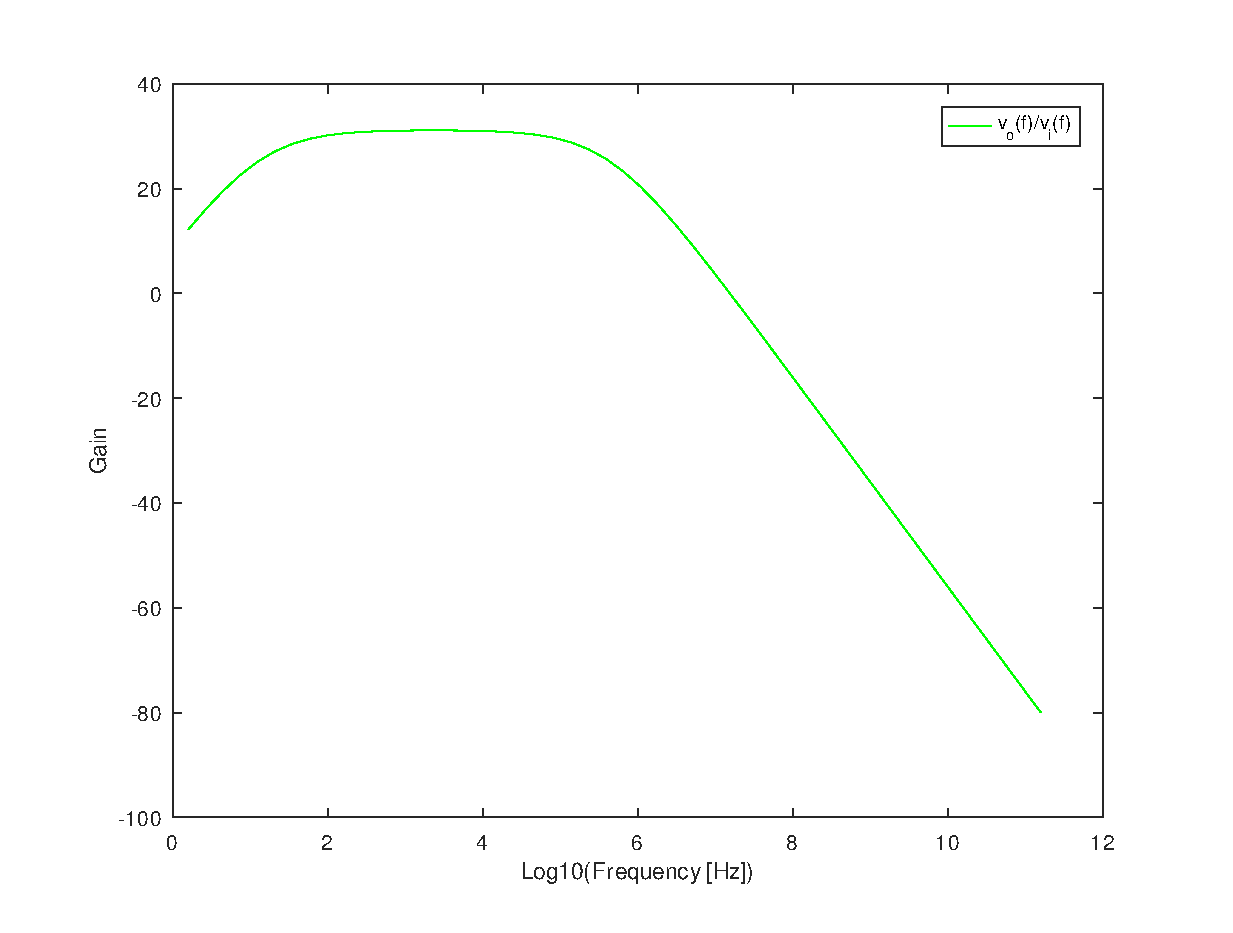
\includegraphics[width = 8cm]{Gain.eps} 
\caption{Gain}
\label{gain}
\end{figure}

By analysing the figure \ref{gain}, we can see that there are 3 types of elements: a NPN BJT, resistors and capacitors.
The first capacitor, $C_in$ , is a coupling capacitor, that acts as a DC Block, so that $V_in$ doesn’t
introduce a DC component of 0, that would change the Operating Point (OP) of the transistor.
The second capacitor, $C _E$ , acts as a bypass capacitor, for it ensures that for low frequencies
all the current flows through $R_E$, and for high frequencies, it passes through the capacitor.
Generally, the output impedance of this stage is high, when compared with the load,
being this the major reason why we cant use just this stage, and we need another one. \par
Both of the capacitors are being analysed in the section of Simulation Analysis.




\subsubsection{Inspection analysis}

From the simulation results we know that the voltage gain curve is maximum for medium frequencies. So, in order to analyse this circuit, we start from the inspection analysis, this is, analysing the circuit for the medium frequencies to obtain the maximum voltage gain. 

To make this analysis we start with computing the operating point (OP), to make sure that our trasistors are always operating in the foward active region(FAR). To compute the operating point for the gain stage we use the mesh method, which leeds to the following matrix:

\begin{equation}
\begin{pmatrix}
R_{B1} \parallel R_{B2} & 0 & R_E \\
-\beta_f & 1 & 0 \\
-\beta_f - 1 & 0 & 1 \\ 
\end{pmatrix}
\begin{pmatrix}
I_B\\
I_C\\
I_E
\end{pmatrix}
=
\begin{pmatrix}
\frac{R_{B2}}{R_{B1} + R_{B2}V_{CC} - V_{BEON}}\\
0\\
0
\end{pmatrix}
\centering
\end{equation}

From this matrix we've obtain the following values:

\begin{table}[H] \centering
\begin{tabular}{|
>{\columncolor[HTML]{FFCC67}}l |c|}
\hline
\multicolumn{2}{|l|}{\cellcolor[HTML]{EABD8B}Name - Value} \\ \hline
VCE & 6.700109e+00 V\\ \hline
VBEON & 7.000000e-01 V \\ \hline
IB1 & 5.815111e-06 A \\ \hline
IC1 & 1.039160e-03 A \\ \hline
IE1 & 1.044976e-03 A \\ \hline

\end{tabular}
\caption{optab}
\end{table}

Which indicate that the transistor is always operating in the FAR.

After this we procede to the incremental analysis, which we'll determine what is the actual voltage gain from the gain stage. The incremental circuit that is going to be analysed, the circuit for medium frequencies where the capacitor $C_e$ is like a short circuit is the following:

\begin{figure}[H] 
\centering
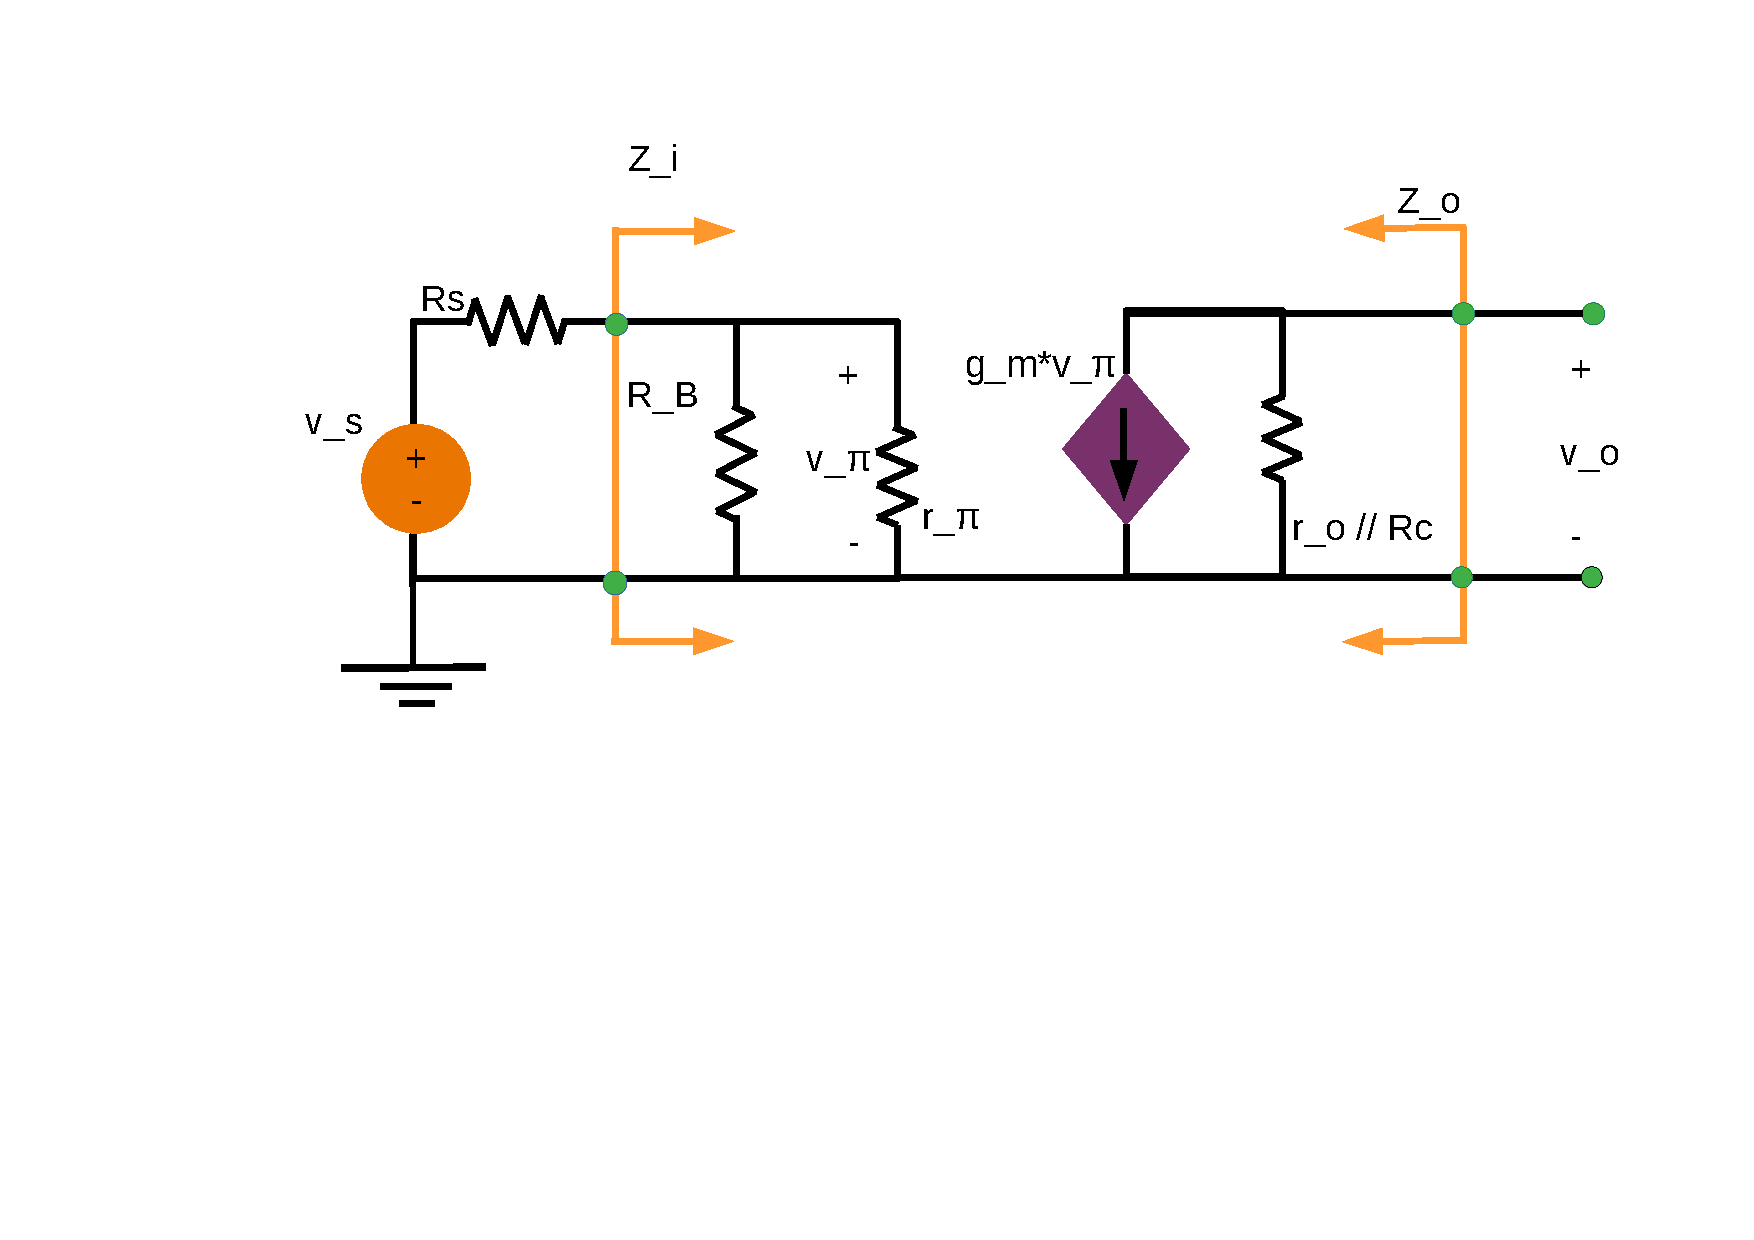
\includegraphics[width = 8cm]{Incremental_Gain.pdf} 
\caption{Output}
\label{output}
\end{figure}

Using the mesh method again, the expression for the voltage gain is presented below:

\begin{equation}
\frac{v_o}{v_i} = -g_m(R_C \parallel r_o)\frac{R_{B1} \parallel R_{B2} \parallel r_{\pi 1}}{R_S + R_{B1} \parallel R_{B2} \parallel r_{\pi 1}}
\end{equation} 

For the output stage we use the same procedure and its OP results are presented below:

\begin{table}[H] \centering
\begin{tabular}{|
>{\columncolor[HTML]{FFCC67}}l |c|}
\hline
\multicolumn{2}{|l|}{\cellcolor[HTML]{EABD8B}Name - Value} \\ \hline
VEC & 7.504614e+00 V\\ \hline
VEBON & 7.000000e-01 V \\ \hline
IB2 & -3.284384e-05 A \\ \hline
IC2 & 7.465405e-03 A \\ \hline
IE2 & 7.498249e-03 A \\ \hline

\end{tabular}
\caption{optab}
\end{table}

Which means that the transistor is always operating in the FAR.

For the voltage gain in this stage, table below presents all the gains for the 2 stages and for the complete circuit.

\subsubsection{Impedances}

In the thereotical analysis of the impedances, we will evaluate the four impedances associated with the two
stages ($Z_in1$ \& $Z_out1$ for the first stage, $Z_in2$ \& $Z_out2$ for the second stage) as well as the two gains associated with each stage ($A_V1$ and $A_V2$, respectively). To do so, we need to perform an Operating Point Analysis to find the values necessary or the Incremental Analysis. \par
In the Gain stage, the input ($Z_in$) and output ($Z_out$) impedances can be derived by the Kirchoff Laws.
Giving us the following equation, where $R_B$ = $R_1$ // $R_2$

\begin{equation}
    Z_{in1}=R_B // r_{\pi 1}
\end{equation}

Due to the presence of the bypass capacitor and to the theoretical approach where it is assumed that the capacitors are short-circuited, we consider $R_E$ approximately 0. It is important to say that the Gain Stage input impedance matches also with the total input impedance of the circuit, as this stage is load-independent. \par
On the other hand, the first stage output impedance can be obtained by:

\begin{equation}
Z_{out1} = {r_o}//{R_{C}}
\label{eq3}
\end{equation} 

Refering the second stage, by analysing the circuit we get:

\begin{equation}
    Z_{in2}=\frac{(g_{m2}+g_{\pi2}+g_{o2}+g_{E2})}{g_{\pi2}(g_{\pi2}+g_{o2}+g_{E2})}
\end{equation}

\begin{equation}
    Z_{out2}=\frac{1}{(g_{m2}+g_{\pi2}+g_{o2}+g_{E2})}
\end{equation}

And finally, the total output impedance is calculated as the following:

\begin{equation}
    Z_{Out}=\frac{v_o}{i_o}=\frac{1}{g_{o2}+g_{m2}\frac{r_{\pi2}}{r_{\pi2}+Z_{out1}}+g_{E2}+\frac{1}{r_{\pi2}+Z_{out1}}}
\end{equation}

The 4 values are presented below,

\begin{table}[H] \centering
\begin{tabular}{|
>{\columncolor[HTML]{FFCC67}}l |c|}
\hline
\multicolumn{2}{|l|}{\cellcolor[HTML]{EABD8B}Name - Value} \\ \hline
ZI1 & 2.419648e+03 Omega \\ \hline
ZO1 & 4.652785e+03 Omega \\ \hline

\end{tabular}
\caption{optab}
\end{table}

Regarding to the compatibility between both stages, remembering that $Z_{out1}$ needs to be  much lower than $Z_{in2}$, we have satisfactory results, in order so that there is no signal degradation or loss between these stages. We can clearly affirm that $V_{in2}$ needs to be as close as possible to $V_{out2}$, confirmed if we apply a voltage divider with $Z_{in2}>>Z_{out1}$:

\begin{equation}
    V_{in2} = \frac{Z_{in2}}{Z_{in2}+Z_{out1}} V_{out2}. 
\end{equation}

\subsubsection{Cutoff frequencies}

After obtaining the gain for the medium frequencies we need to determine the frequency dependance of this gain. To do so we've used two methods called short circuit time constant (SCTC) and open circuit time constant (OCTC). The SCTC was used in the determination of the lower cutoff frequency and it consists in the determination of the equivalent resistance seen by all capacitors individually using the in the following steps:

\begin{itemize}

\item Short-Circuit all large Capacitors that are not being analysed 
\item Replace the capacitor that is being analysed by a test voltage source
\item Remove all the independant sources(Short-circuit the independant voltage sources and open-circuit the independant current sources) 
\item Open-circuit all the small capacitors

\end{itemize}

by large capacitors we mean the capacitors implemented in the circuit and by small capacitors we mean the capacitors associated with the transistor.

After doing this steps, we use the dominant pole aproximation, which converts all poles of the graphic in just the one that has the most influence in the graphic. By these aproximation, the lower cutoff frequency is given by:

\begin{equation}
w_L = \sum_{n = 1}^n \frac{1}{R_{iS}C_i}
\label{wl}
\end{equation} 

Being n the number of large capacitors.

Proceding as described we've obtained the following expressions for the equivalent resistances:

\begin{equation}
R_{eq_{in}} = R_{in} + Z_{In1}
\end{equation} 

\begin{equation}
R_{eq_{E}} = \frac{1}{\frac{1}{R_E}+\frac{1+g_mr_{\pi 1}}{R_S \parallel R_B + r_{\pi 1}}}
\end{equation} 

\begin{equation}
R_{eq_{in}} = R_{L} + Z_{Out2}
\end{equation} 

So using the formulae \ref{wl} we've obtained the lower cutoff frequency.

Moving on to the higher cutoff frequency, we now have to use the OCTC, which has the same steps as the SCTC, but now we analyse the small capacitors associated with the transistor($C_{\pi}$ $C_{o}$). Another difference is the formulae associated with the dominant pole aproxiamtion, which is:

\begin{equation}
w_H = \frac{1}{\sum_{n = 1}^n R_{iS}C_i}
\label{wh}
\end{equation} 

so doing the OCTC we get:

\begin{equation}
R_{eq_{\pi}} = r_{\pi 1}
\end{equation} 

\begin{equation}
R_{eq_{o}} = r_{o}
\end{equation} 

And once more using the formulae \ref{wh} we've obtained the higher cutoff frequency.

\begin{table}[H] \centering
\begin{tabular}{|
>{\columncolor[HTML]{FFCC67}}l |c|}
\hline
\multicolumn{2}{|l|}{\cellcolor[HTML]{EABD8B}Name - Value} \\ \hline
HighCutOff frequency & 8.304945e+05 Hz\\ \hline
LowCutOff frequency & 2.183854e+01 Hz\\ \hline
Bandwidth & 8.304726e+05 rad/s\\ \hline

\end{tabular}
\caption{optab}
\end{table}



\subsection{Output stage}

As we could see in the section of the Gain stage, we end up with a high output impedance $Z_O1$ . For that reason, we
connect a second circuit to the output of the Gain Stage, that produce a low output impedance.
This part of the stage is presented in the figure below:

\begin{figure}[H] 
\centering
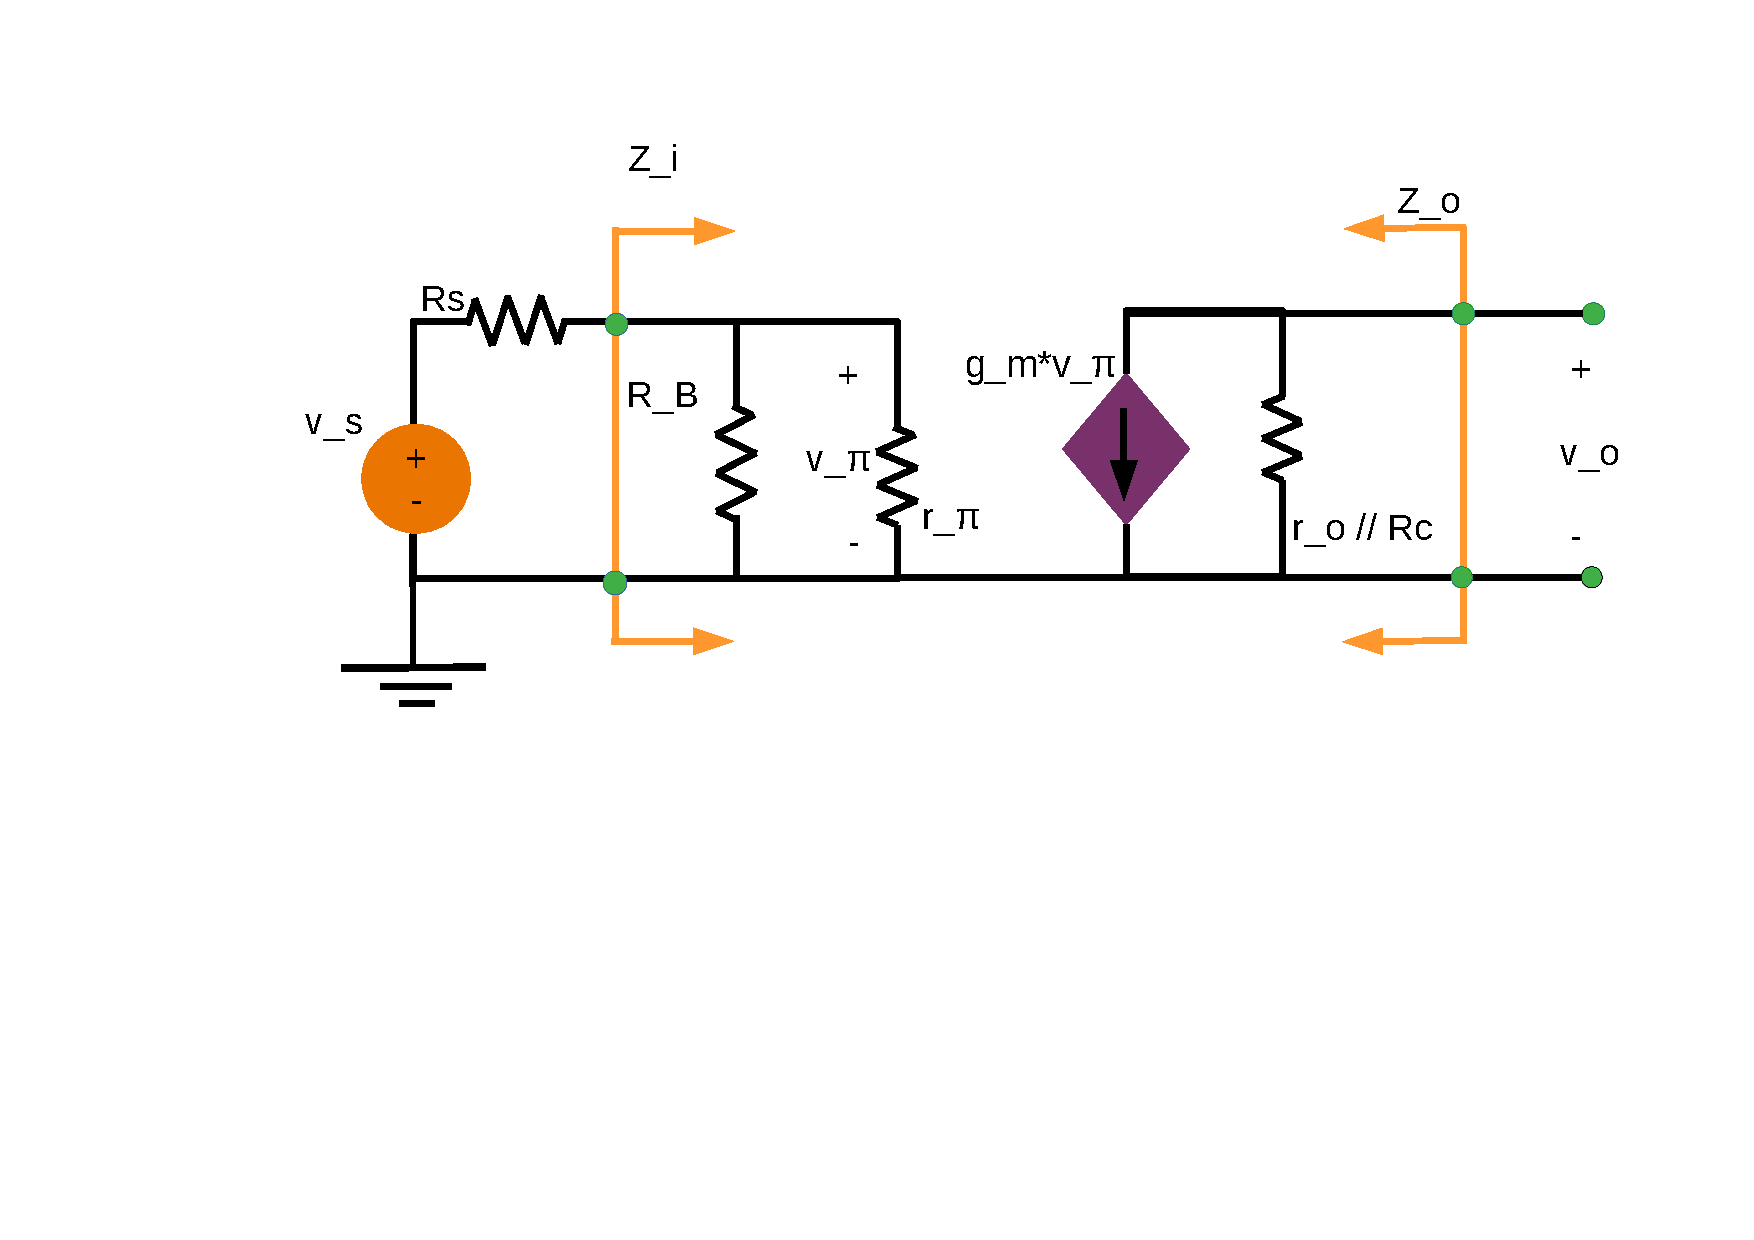
\includegraphics[width = 8cm]{Incremental_Gain.pdf} 
\caption{Output}
\label{output}
\end{figure}

By analysing the figure, we can conclude that this circuit presents similar components but with some differences.
Instead of a NPN BJT, we use a PNP BJT, because it has a higher $\beta_F$, that lowers the
output impedance as we desire. It also illustrates the use of another BJT transistor. \par
Another capacitor, $C_o$ , is used with a similar goal as the previous coupling capacitor. If we
didn’t use this component, the gain stage would introduce a DC voltage of 0 to the second stage,
which as previous would change and ruin the transistor’s Operating Point. \par
We will end up with a lower output impedance in this stage, when compared to
the load, and a higher input impedance when compared to the output impedance of the gain
stage. When we combine both stages, we need to ensure that there is a compatibility between the
impedances of both stages. In fact, by the voltage divider law, to make sure no voltage signal is lost, the input
impedance of the second stage should be much greater than the output impedance of the first
one.\par

\begin{table}[H] \centering
\begin{tabular}{|
>{\columncolor[HTML]{FFCC67}}l |c|}
\hline
\multicolumn{2}{|l|}{\cellcolor[HTML]{EABD8B}Name - Value} \\ \hline
ZI2 & 4.075483e+04 Omega \\ \hline
ZO2 & 1.478440e+00 Omega \\ \hline

\end{tabular}
\caption{optab}
\end{table}

To conclude, when we merge these two circuits, we end up with the BJT Audio Amplifier represented in Figure 1.

\begin{table}[H] \centering
\begin{tabular}{|
>{\columncolor[HTML]{FFCC67}}l |c|}
\hline
\multicolumn{2}{|l|}{\cellcolor[HTML]{EABD8B}Name - Value} \\ \hline
VoltageGain1& 2.075755e+01 V\\ \hline
VoltageGain2 & 9.916852e-01 V\\ \hline
VoltageGain & 1.980831e+01 V\\ \hline

\end{tabular}
\caption{optab}
\end{table}



%\begin{table}[H] \centering
%\begin{tabular}{|
%>{\columncolor[HTML]{FFCC67}}l |c|}
%\hline
%\multicolumn{2}{|l|}{\cellcolor[HTML]{EABD8B}Name - Value} \\ \hline
%@cb[i] & 0.000000e+00\\ \hline
@ce[i] & 0.000000e+00\\ \hline
@q1[ib] & 7.022567e-05\\ \hline
@q1[ic] & 1.404513e-02\\ \hline
@q1[ie] & -1.41154e-02\\ \hline
@q1[is] & 5.765392e-12\\ \hline
@rc[i] & 1.411536e-02\\ \hline
@re[i] & 1.411536e-02\\ \hline
@rf[i] & 7.022567e-05\\ \hline
@rs[i] & 0.000000e+00\\ \hline
v(1) & 0.000000e+00\\ \hline
v(2) & 0.000000e+00\\ \hline
base & 2.254108e+00\\ \hline
coll & 5.765392e+00\\ \hline
emit & 1.411536e+00\\ \hline
vcc & 1.000000e+01\\ \hline

%\end{tabular}
%\caption{optab}
%\end{table}

%\begin{table}[H] \centering
%\begin{tabular}{|
%>{\columncolor[HTML]{FFCC67}}l |c|}
%\hline
%\multicolumn{2}{|l|}{\cellcolor[HTML]{EABD8B}Name - Value} \\ \hline
%First Stage\\ \hline
AV1-DB & 2.634352e+01 dB\\ \hline
ZI1 & 2.811209e+03 Omega \\ \hline
ZO1 & 3.754073e+03 Omega \\ \hline
Second Stage\\ \hline
AV2-DB & -7.252308e-02 dB\\ \hline
ZI2 & 4.075483e+04 Omega \\ \hline
ZO2 & 1.478440e+00 Omega \\ \hline
Complete\\ \hline
ZO & 1.710806e+01 Omega\\ \hline
AV-DB & 2.593695e+01 dB\\ \hline
Merit & 4.398471e+02 \\ \hline
HighCutOff frequency & 8.304945e+05 Hz\\ \hline
LowCutOff frequency & 2.183854e+01 Hz\\ \hline
Cost & 2.242430e+03 MU's\\ \hline
Bandwidth & 8.304726e+05 rad/s\\ \hline

%\end{tabular}
%\caption{Point 2}
%\end{table}

